\chapter{Hauptteil}
Der Hauptteil besteht üblicherweise aus mehreren Kapiteln, die verschiedene Aspekte der Arbeit beleuchten. Es ist ratsam für jedes Kapitel ein eigene Tex-Datei anzulegen, damit der Quellcode übersichtlich bleibt. Prinzipiell gibt es für wissenschaftliche Arbeiten bzw. wissenschaftliches Schreiben einen grundlegenden \glqq Bauplan\grqq{}:
\begin{enumerate}
    \item Einführung (Introduction) - Welches Themengebiet behandelt die Arbeit und warum? Was sind die Ziele?
    \item Stand der Technik (Related Work) - Welche Arbeiten und verwandte Forschungsprojekte gibt es in diesem Themengebiet bereits?
    \item Grundlagen (Background) - Welche Grundlagen bilden das Fundament der Arbeit und werden zum Verständnis benötigt?
    \item Umsetzung (Design and Implementation) - Dies ist das Hauptkapitel. Das Kapitel wird entsprechend des Arbeitsthemas angepasst, je nach dem ob man im Rahmen der Arbeit beispielsweise etwas selbstständig entwickelt (Software, Hardware, sonstiges) oder eine Literaturanalyse durchführt (usw.). Fragestellung: Was mache ich im Rahmen meiner Arbeit und wie wird dies realisiert?
    \item Experimentelle Validierung (Evaluation) - Falls praktische Experimente wie etwa Benchmarks oder Systemtests im Rahmen einer Arbeit Sinn machen: Wie sieht mein Testaufbau aus? Welche Experimente werden durchgeführt? Was sind die Ergebnisse und wie interpretiere ich diese?
    \item Schlussbetrachtungen (Conclusion) - Zusammenfassung der Arbeit und Ausblick auf mögliche Folgearbeiten.
\end{enumerate}
Je nach dem um welche Art des wissenschaftlichen Schreibens (z.B. Abschlussarbeit, Seminararbeit, Bericht zu Forschungsprojekt, Fachartikel / Paper, etc.) es sich handelt, kann der \glqq Bauplan\grqq{} entsprechend angepasst werden.

\section{Verwendung dieser Vorlage}
Dieses Template ist für die Verwendung mit pdflatex gedacht. Am einfachsten ist es die Vorlage in Overleaf \cite{overleaf} zu öffnen. Overleaf ist eine Onlineanwendung zum Arbeiten mit \LaTeX{}, was den Vorteil hat, dass nichts lokal installiert werden muss und mit jedem Betriebssystem gearbeitet werden kann, das über einen Browser verfügt. Außerdem ist es möglich mit mehreren Personen gemeinsam an einem Projekt zu arbeiten. Die Vorlage kann auch mit einer lokalen Installation verwendet werden. Die Website von Overleaf bietet zudem einige gute Tutorials zum Arbeiten mit \LaTeX{}: \url{https://www.overleaf.com/learn}.

Fehler und Warnungen, die beim Compilieren erzeugt werden, sollten direkt behoben werden, da es später schwierig sein kann den eigentlichen Auslöser einer Fehlermeldung zu finden. Manchmal sieht das Dokument trotz Fehlermeldung oder Warnung korrekt aus, der Fehler macht sich dann aber später bemerkbar. Die Meldungen sind leider oft nicht sehr aussagekräftig, weshalb es am einfachsten ist direkt nach dem Auftreten eines Fehlers den Teil der Arbeit anzuschauen, der als letztes geändert wurde.

\section{Unterkapitel}
Unterkapitel sollten ein abgeschlossenes Thema behandeln. Einzelne Unterkapitel in einem Kapitel sind zu vermeiden, also z.\,B. in Kapitel 2 das Unterkapitel 2.1, aber kein weiteres Unterkapitel. In diesem Fall ist es besser entweder den Inhalt von 2.1 direkt in Kapitel 2 zu schreiben, oder falls 2 und 2.1 thematisch zu weit voneinander entfernt sind, aus Unterkapitel 2.1 ein eigenes Kapitel 3 zu machen.

\section{Grafiken}
In der Informatik sind die häufigsten Grafiken entweder Diagramme oder Plots. Beide Arten von Grafiken lassen sich gut als Vektorgrafiken erstellen und einbinden. Der Vorteil von Vektor- gegenüber Pixelgrafiken ist, dass beliebig weit in eine Grafik hereingezoomt werden kann, ohne dass sie unscharf wird. Zudem benötigen Vektorgrafiken meistens weniger Speicherplatz.

Grafiken können direkt in \LaTeX{} mit dem TikZ Paket \cite{tikz} erstellt werden. Die Verwendung ist etwas gewöhnungsbedürftig, da Grafiken mit Code beschrieben werden, bietet aber viele Freiheiten. Außerdem werden die so erstellten Grafiken direkt in \LaTeX{} gerendert und verwenden die selbe Schriftart wie im Text und eine konsistente Schriftgröße im gesamten Dokument. Ein weiteres beliebtes Programm zum Erstellen von Vektorgrafiken ist Inkscape \cite{inkscape}. Zudem bieten viele Programme die Möglichkeit eine Grafik z.\,B. als PDF zu exportieren, was in \LaTeX{} als Vektorgrafik eingebunden werden kann.

Pixelgrafiken lassen sich nicht immer vermeiden, z.\,B. wenn eine Foto in die Arbeit eingebunden werden soll. In diesem Fall sollte darauf geachtet werden, dass die Grafik über eine ausreichende Auflösung verfügt. Eine Auflösung von 300~dpi ist ein guter Richtwert, um beim Drucken ein gutes Ergebnis zu erhalten.

Abbildungen \ref{fig:ieee_float_format_vector} und \ref{fig:ieee_float_format_pixel} zeigen beide den Aufbau des IEEE Floating Point Formats. Abbidlung \ref{fig:ieee_float_format_pixel} ist eine Pixelgrafik, während Abbildung \ref{fig:ieee_float_format_vector} mit TikZ erstellt wurde. Der Unterschied wird beim hereinzoomen deutlich.

\begin{figure}[ht]
\centering
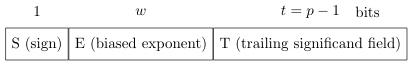
\includegraphics[width=0.65\textwidth]{figures/ieee_float_format.jpg}
\caption{Aufbau des IEEE Floating Point Formats als Pixelgrafik.}
\label{fig:ieee_float_format_pixel}
\end{figure}

\section{Tabellen}
Tabellen können in \LaTeX{} direkt erstellt werden. Tabelle \ref{tab:ieee_formats} zeigt ein Beispiel dafür. Einfache Tabellen lassen sich schnell erstellen, bei komplizierteren Tabellen ist es manchmal einfacher zusätzliche Pakete zu verwenden. Mit dem Paket multirow \cite{multirow} können z.\,B. einfacher Tabellen erstellt werden, bei denen einzelne Zeilen oder Spalten zusammengefasst sind.

\begin{table}[ht]
\centering
\begin{tabular}{|l|r|r|r|r|} 
 \hline
 Parameter & binary16 & binary32 & binary64 & binary128 \\
 \hline
  $k$, storage width in bits           & 16 &  32 &   64 &   128 \\ 
  $w$, exponent field width in bits    &  5 &   8 &   11 &    15 \\
  $t$, significand field width in bits & 10 &  23 &   52 &   112 \\
  emax, maximum exponent $e$           & 15 & 127 & 1023 & 16383 \\
  bias, $E-e$                          & 15 & 127 & 1023 & 16383 \\
 \hline
\end{tabular}
\caption{IEEE 754-2019 Floating Point Formate als Beispiel für das Einbinden einer Tabelle.}
\label{tab:ieee_formats}
\end{table}

\section{Quellcode}
Um Quellcode in die Arbeit einzubinden, können in \LaTeX{} Listings verwendet werden. Es gibt für populäre Sprachen vorgefertigte Umgebungen, welche die Syntax farblich hervorheben. Quellcode sollte eingebunden werden, wenn eine konkrete Implementierung in einer Sprache erläutert wird. Für die Erklärung eines Algorithmus ist es oft übersichtlicher ein Schaubild oder Pseudocode zu verwenden. Es sollten nur kurze Codeabschnitte eingebunden werden, die für den Leser einfach nachvollziehbar sind und nur den für die Erklärung relevanten Code enthalten. Längere Codeabschnitte können im Anhang stehen. Der komplette Code, der für die Arbeit geschrieben wurde, sollte in einem Repository abgelegt werden.

Listing \ref{lst:example_listing} zeigt ein Beispiel für ein Codelisting in der Programmiersprache C. Algorithmus \ref{alg:west} zeigt einen Routing Algorithmus als Pseudocode. Der Code wurde mit dem Paket algorithm2e \cite{algorithm2e} erstellt.

\begin{lstlisting}[language=C, caption=Beispiel für ein Codelisting in der Sprache C., label=lst:example_listing]
#include <stdio.h>
// comments are highlighted in green
void main() {
    // keywords of the language are highlighted in blue
    for (int i = 0; i <= 42; ++i) {
        printf("%d\n", i);
    }
    // strings are highlighted in red
    printf("Hello World!");
}
\end{lstlisting}

\begin{algorithm}[ht]

    \uIf{destination in west direction}{
        go West;
    }
    \uElseIf{destination in same column}{
        \eIf{destination in north direction}{
            go North;
        }{
            go South;
        }
    }
    \uElseIf{destination in north east direction}{
        go North or go East
    }
    \uElseIf{destination in south east direction}{
        go South or go East
    }
    \uElseIf{destination in same row and in east direction}{
        go East;
    }
    \uElseIf{at destination}{
        done;
}
 \caption{West First-Routing Algorithm.}
 \label{alg:west}
\end{algorithm}

\section{Literatur}
Ein Literaturverzeichnis kann z.B. mit dem Bibtex Paket \cite{bibtex} erstellt werden. Dazu wird für jede Quelle ein Eintrag in der Datei \texttt{references.bib} angelegt. An der passenden Stelle im Text können diese Einträge mit dem \ensuremath{\backslash} cite\{\} Befehl zitiert werden. Für jede Quelle die zitiert wird, legt \LaTeX{}  im Literaturverzeichnis einen Eintrag an.

Beschreibungen der Quellen im Bibtex-Format müssen meistens nicht selbst erstellt werden, sondern können direkt bei vielen Verlagen und Bibliotheken direkt generiert werden. Wissenschaftliche Softwareprojekte geben ebenfalls oft auf ihrer Website eine Beschreibung im Bibtex-Format an.



\section{Abkürzungen}
Für jede verwendete Abkürzung kann ein Eintrag in der Datei \texttt{acronyms.tex} angelegt werden. Wenn diese Abkürzung im Text zum ersten Mal auftaucht, sollte der Begriff ausgeschrieben werden mit der Abkürzung in Klammern dahinter. Bei weiteren Vorkommen im Text kann dann die eigentliche Abkürzung verwendet werden. In \LaTeX{} gibt es dafür spezielle Befehle. Beispiel für ausgeschriebene Abkürzung (siehe Quelltext des Dokuments für die entsprechenden Befehle): \acrfull{nic}. Beispiel für das Verwenden der Abkürzung: \acrshort{nic}. Die verwendeten Abkürzungen werden automatisch im Abkürzungsverzeichnis aufgelistet.
